% Options for packages loaded elsewhere
\PassOptionsToPackage{unicode}{hyperref}
\PassOptionsToPackage{hyphens}{url}
\PassOptionsToPackage{dvipsnames,svgnames,x11names}{xcolor}
%
\documentclass[
  letterpaper,
  DIV=11,
  numbers=noendperiod]{scrreprt}

\usepackage{amsmath,amssymb}
\usepackage{iftex}
\ifPDFTeX
  \usepackage[T1]{fontenc}
  \usepackage[utf8]{inputenc}
  \usepackage{textcomp} % provide euro and other symbols
\else % if luatex or xetex
  \usepackage{unicode-math}
  \defaultfontfeatures{Scale=MatchLowercase}
  \defaultfontfeatures[\rmfamily]{Ligatures=TeX,Scale=1}
\fi
\usepackage{lmodern}
\ifPDFTeX\else  
    % xetex/luatex font selection
\fi
% Use upquote if available, for straight quotes in verbatim environments
\IfFileExists{upquote.sty}{\usepackage{upquote}}{}
\IfFileExists{microtype.sty}{% use microtype if available
  \usepackage[]{microtype}
  \UseMicrotypeSet[protrusion]{basicmath} % disable protrusion for tt fonts
}{}
\makeatletter
\@ifundefined{KOMAClassName}{% if non-KOMA class
  \IfFileExists{parskip.sty}{%
    \usepackage{parskip}
  }{% else
    \setlength{\parindent}{0pt}
    \setlength{\parskip}{6pt plus 2pt minus 1pt}}
}{% if KOMA class
  \KOMAoptions{parskip=half}}
\makeatother
\usepackage{xcolor}
\setlength{\emergencystretch}{3em} % prevent overfull lines
\setcounter{secnumdepth}{5}
% Make \paragraph and \subparagraph free-standing
\ifx\paragraph\undefined\else
  \let\oldparagraph\paragraph
  \renewcommand{\paragraph}[1]{\oldparagraph{#1}\mbox{}}
\fi
\ifx\subparagraph\undefined\else
  \let\oldsubparagraph\subparagraph
  \renewcommand{\subparagraph}[1]{\oldsubparagraph{#1}\mbox{}}
\fi

\usepackage{color}
\usepackage{fancyvrb}
\newcommand{\VerbBar}{|}
\newcommand{\VERB}{\Verb[commandchars=\\\{\}]}
\DefineVerbatimEnvironment{Highlighting}{Verbatim}{commandchars=\\\{\}}
% Add ',fontsize=\small' for more characters per line
\usepackage{framed}
\definecolor{shadecolor}{RGB}{241,243,245}
\newenvironment{Shaded}{\begin{snugshade}}{\end{snugshade}}
\newcommand{\AlertTok}[1]{\textcolor[rgb]{0.68,0.00,0.00}{#1}}
\newcommand{\AnnotationTok}[1]{\textcolor[rgb]{0.37,0.37,0.37}{#1}}
\newcommand{\AttributeTok}[1]{\textcolor[rgb]{0.40,0.45,0.13}{#1}}
\newcommand{\BaseNTok}[1]{\textcolor[rgb]{0.68,0.00,0.00}{#1}}
\newcommand{\BuiltInTok}[1]{\textcolor[rgb]{0.00,0.23,0.31}{#1}}
\newcommand{\CharTok}[1]{\textcolor[rgb]{0.13,0.47,0.30}{#1}}
\newcommand{\CommentTok}[1]{\textcolor[rgb]{0.37,0.37,0.37}{#1}}
\newcommand{\CommentVarTok}[1]{\textcolor[rgb]{0.37,0.37,0.37}{\textit{#1}}}
\newcommand{\ConstantTok}[1]{\textcolor[rgb]{0.56,0.35,0.01}{#1}}
\newcommand{\ControlFlowTok}[1]{\textcolor[rgb]{0.00,0.23,0.31}{#1}}
\newcommand{\DataTypeTok}[1]{\textcolor[rgb]{0.68,0.00,0.00}{#1}}
\newcommand{\DecValTok}[1]{\textcolor[rgb]{0.68,0.00,0.00}{#1}}
\newcommand{\DocumentationTok}[1]{\textcolor[rgb]{0.37,0.37,0.37}{\textit{#1}}}
\newcommand{\ErrorTok}[1]{\textcolor[rgb]{0.68,0.00,0.00}{#1}}
\newcommand{\ExtensionTok}[1]{\textcolor[rgb]{0.00,0.23,0.31}{#1}}
\newcommand{\FloatTok}[1]{\textcolor[rgb]{0.68,0.00,0.00}{#1}}
\newcommand{\FunctionTok}[1]{\textcolor[rgb]{0.28,0.35,0.67}{#1}}
\newcommand{\ImportTok}[1]{\textcolor[rgb]{0.00,0.46,0.62}{#1}}
\newcommand{\InformationTok}[1]{\textcolor[rgb]{0.37,0.37,0.37}{#1}}
\newcommand{\KeywordTok}[1]{\textcolor[rgb]{0.00,0.23,0.31}{#1}}
\newcommand{\NormalTok}[1]{\textcolor[rgb]{0.00,0.23,0.31}{#1}}
\newcommand{\OperatorTok}[1]{\textcolor[rgb]{0.37,0.37,0.37}{#1}}
\newcommand{\OtherTok}[1]{\textcolor[rgb]{0.00,0.23,0.31}{#1}}
\newcommand{\PreprocessorTok}[1]{\textcolor[rgb]{0.68,0.00,0.00}{#1}}
\newcommand{\RegionMarkerTok}[1]{\textcolor[rgb]{0.00,0.23,0.31}{#1}}
\newcommand{\SpecialCharTok}[1]{\textcolor[rgb]{0.37,0.37,0.37}{#1}}
\newcommand{\SpecialStringTok}[1]{\textcolor[rgb]{0.13,0.47,0.30}{#1}}
\newcommand{\StringTok}[1]{\textcolor[rgb]{0.13,0.47,0.30}{#1}}
\newcommand{\VariableTok}[1]{\textcolor[rgb]{0.07,0.07,0.07}{#1}}
\newcommand{\VerbatimStringTok}[1]{\textcolor[rgb]{0.13,0.47,0.30}{#1}}
\newcommand{\WarningTok}[1]{\textcolor[rgb]{0.37,0.37,0.37}{\textit{#1}}}

\providecommand{\tightlist}{%
  \setlength{\itemsep}{0pt}\setlength{\parskip}{0pt}}\usepackage{longtable,booktabs,array}
\usepackage{calc} % for calculating minipage widths
% Correct order of tables after \paragraph or \subparagraph
\usepackage{etoolbox}
\makeatletter
\patchcmd\longtable{\par}{\if@noskipsec\mbox{}\fi\par}{}{}
\makeatother
% Allow footnotes in longtable head/foot
\IfFileExists{footnotehyper.sty}{\usepackage{footnotehyper}}{\usepackage{footnote}}
\makesavenoteenv{longtable}
\usepackage{graphicx}
\makeatletter
\def\maxwidth{\ifdim\Gin@nat@width>\linewidth\linewidth\else\Gin@nat@width\fi}
\def\maxheight{\ifdim\Gin@nat@height>\textheight\textheight\else\Gin@nat@height\fi}
\makeatother
% Scale images if necessary, so that they will not overflow the page
% margins by default, and it is still possible to overwrite the defaults
% using explicit options in \includegraphics[width, height, ...]{}
\setkeys{Gin}{width=\maxwidth,height=\maxheight,keepaspectratio}
% Set default figure placement to htbp
\makeatletter
\def\fps@figure{htbp}
\makeatother
% definitions for citeproc citations
\NewDocumentCommand\citeproctext{}{}
\NewDocumentCommand\citeproc{mm}{%
  \begingroup\def\citeproctext{#2}\cite{#1}\endgroup}
\makeatletter
 % allow citations to break across lines
 \let\@cite@ofmt\@firstofone
 % avoid brackets around text for \cite:
 \def\@biblabel#1{}
 \def\@cite#1#2{{#1\if@tempswa , #2\fi}}
\makeatother
\newlength{\cslhangindent}
\setlength{\cslhangindent}{1.5em}
\newlength{\csllabelwidth}
\setlength{\csllabelwidth}{3em}
\newenvironment{CSLReferences}[2] % #1 hanging-indent, #2 entry-spacing
 {\begin{list}{}{%
  \setlength{\itemindent}{0pt}
  \setlength{\leftmargin}{0pt}
  \setlength{\parsep}{0pt}
  % turn on hanging indent if param 1 is 1
  \ifodd #1
   \setlength{\leftmargin}{\cslhangindent}
   \setlength{\itemindent}{-1\cslhangindent}
  \fi
  % set entry spacing
  \setlength{\itemsep}{#2\baselineskip}}}
 {\end{list}}
\usepackage{calc}
\newcommand{\CSLBlock}[1]{\hfill\break\parbox[t]{\linewidth}{\strut\ignorespaces#1\strut}}
\newcommand{\CSLLeftMargin}[1]{\parbox[t]{\csllabelwidth}{\strut#1\strut}}
\newcommand{\CSLRightInline}[1]{\parbox[t]{\linewidth - \csllabelwidth}{\strut#1\strut}}
\newcommand{\CSLIndent}[1]{\hspace{\cslhangindent}#1}

\KOMAoption{captions}{tableheading}
\makeatletter
\@ifpackageloaded{bookmark}{}{\usepackage{bookmark}}
\makeatother
\makeatletter
\@ifpackageloaded{caption}{}{\usepackage{caption}}
\AtBeginDocument{%
\ifdefined\contentsname
  \renewcommand*\contentsname{Table of contents}
\else
  \newcommand\contentsname{Table of contents}
\fi
\ifdefined\listfigurename
  \renewcommand*\listfigurename{List of Figures}
\else
  \newcommand\listfigurename{List of Figures}
\fi
\ifdefined\listtablename
  \renewcommand*\listtablename{List of Tables}
\else
  \newcommand\listtablename{List of Tables}
\fi
\ifdefined\figurename
  \renewcommand*\figurename{Figure}
\else
  \newcommand\figurename{Figure}
\fi
\ifdefined\tablename
  \renewcommand*\tablename{Table}
\else
  \newcommand\tablename{Table}
\fi
}
\@ifpackageloaded{float}{}{\usepackage{float}}
\floatstyle{ruled}
\@ifundefined{c@chapter}{\newfloat{codelisting}{h}{lop}}{\newfloat{codelisting}{h}{lop}[chapter]}
\floatname{codelisting}{Listing}
\newcommand*\listoflistings{\listof{codelisting}{List of Listings}}
\makeatother
\makeatletter
\makeatother
\makeatletter
\@ifpackageloaded{caption}{}{\usepackage{caption}}
\@ifpackageloaded{subcaption}{}{\usepackage{subcaption}}
\makeatother
\ifLuaTeX
  \usepackage{selnolig}  % disable illegal ligatures
\fi
\usepackage{bookmark}

\IfFileExists{xurl.sty}{\usepackage{xurl}}{} % add URL line breaks if available
\urlstyle{same} % disable monospaced font for URLs
\hypersetup{
  pdftitle={Evaluation of Possible Sharknados},
  pdfauthor={Jesus Rodriguez},
  colorlinks=true,
  linkcolor={blue},
  filecolor={Maroon},
  citecolor={Blue},
  urlcolor={Blue},
  pdfcreator={LaTeX via pandoc}}

\title{Evaluation of Possible Sharknados}
\author{Jesus Rodriguez}
\date{}

\begin{document}
\maketitle

\renewcommand*\contentsname{Table of contents}
{
\hypersetup{linkcolor=}
\setcounter{tocdepth}{2}
\tableofcontents
}
\bookmarksetup{startatroot}

\chapter*{Preface}\label{preface}
\addcontentsline{toc}{chapter}{Preface}

\markboth{Preface}{Preface}

You are a data scientist for a mid-sized business, in a small group of
3-4 data scientists. You've been tasked with creating a report
evaluating a scenario for your business. Your colleagues will also be
evaluating the same scenario, and your reports will be used in aggregate
to determine a consensus (or lack thereof) on the company's action. The
reports will also be used to inform downsizing that is rumored to be
coming - you want to ensure your report is better than your peers so
that you aren't as easy to cut.

You may talk to your peers who are assigned the same scenario, but you
do not want to collaborate too closely, lest you both become targets of
the rumored layoffs.

\begin{center}\rule{0.5\linewidth}{0.5pt}\end{center}

I've scaffolded this report for you to make this process easier - as we
talk about different sections of a report in class and read about how to
create similar sections, you will practice by writing the equivalent
section of your report.

The basic steps for this task are as follows:

\begin{itemize}
\tightlist
\item
  Identify the research question from the business question
\end{itemize}

What is the frequency of tornadoes that form in shark infested waters on
the coastline happen to move inwards, and how common is it that these
same tornadoes also have the strength to lift sharks from those waters?

\begin{itemize}
\item
  Identify data set(s) which are (1) publicly available (you don't have
  a budget to pay for private data) and (2) relevant to your task

  \begin{itemize}
  \tightlist
  \item
    (HW Week 6) Document your data sets in \texttt{draft-data-doc.qmd}
  \end{itemize}
\item
  Conduct a statistical analysis to support your answer to your research
  and business questions

  \begin{itemize}
  \item
    Write a methods section for your business report corresponding to
    your statistical analysis
  \item
    (HW Week 9) Draft of results section of business report with
    relevant graphics/visual aids in \texttt{draft-results.qmd}
  \end{itemize}
\item
  Write your report

  \begin{itemize}
  \item
    (HW Week 10) Draft of Intro/Conclusion sections in
    \texttt{draft-intro-conclusions.qmd}
  \item
    (HW Week 11) Draft of Executive summary section in
    \texttt{draft-exec-summary.qmd}
  \end{itemize}
\item
  Revise your report

  \begin{itemize}
  \item
    (HW Week 12 -- not turned in) Revise your report
  \item
    (HW Week 13) - Rough draft of report due. Create one or more qmd
    files for your report (you can overwrite or delete intro.qmd and
    summary.qmd), include the names of each file (in order) in
    \texttt{\_quarto.yml}. You should use references (edit
    references.bib and use pandoc citations). Make sure your report
    compiles and looks reasonable in both html and pdf.
  \item
    Develop a presentation to go along with your report (Week 13).
    Create slides for your report using quarto.
  \end{itemize}
\item
  Peer revise reports

  \begin{itemize}
  \item
    Peer revise reports
  \item
    (HW Week 14) - Make edits to your report from comments received from
    peer review
  \end{itemize}
\item
  Final report \& presentation due
\end{itemize}

\bookmarksetup{startatroot}

\chapter{Introduction}\label{introduction}

\section{Big Picture}\label{big-picture}

\subsection{Who is my audience}\label{who-is-my-audience}

\subsubsection{Boss who is scared of a sharknado could occur in real
life}\label{boss-who-is-scared-of-a-sharknado-could-occur-in-real-life}

\paragraph{Talk about what Tornadoes that form over water are
called}\label{talk-about-what-tornadoes-that-form-over-water-are-called}

\paragraph{Discuss the differences between Tornadoes and
Waterspouts}\label{discuss-the-differences-between-tornadoes-and-waterspouts}

\subparagraph{Explain why these differences
matter}\label{explain-why-these-differences-matter}

\subparagraph{IRL a sharknado would be classified as a Waterspout that
transitions into a tornado when it moves over
land}\label{irl-a-sharknado-would-be-classified-as-a-waterspout-that-transitions-into-a-tornado-when-it-moves-over-land}

A waterspout would then be classified as a tornado

\paragraph{Discuss basic information about the shark population around
coastal
areas}\label{discuss-basic-information-about-the-shark-population-around-coastal-areas}

\section{Establish a niche}\label{establish-a-niche}

\subsection{Problem : Can we predict if a sharknado will ever be possibe
to occur IRL using exisiting data about sharks and
tornadoes}\label{problem-can-we-predict-if-a-sharknado-will-ever-be-possibe-to-occur-irl-using-exisiting-data-about-sharks-and-tornadoes}

\subsection{Gap in Knowledge}\label{gap-in-knowledge}

\subsubsection{Waterspouts are not classified as tornadoes, so many do
not have a Tor F Scale to judge how powerful they
are}\label{waterspouts-are-not-classified-as-tornadoes-so-many-do-not-have-a-tor-f-scale-to-judge-how-powerful-they-are}

\subsubsection{Using shark data that is from a different time period of
our Tornado
Data??}\label{using-shark-data-that-is-from-a-different-time-period-of-our-tornado-data}

\section{Occupy a Niche}\label{occupy-a-niche}

\subsection{How does the work approach the niche that's been
identified}\label{how-does-the-work-approach-the-niche-thats-been-identified}

\subsection{What approaches are being
used}\label{what-approaches-are-being-used}

\subsubsection{Not detailed methods, but past literature on how those
methods were established may be
useful}\label{not-detailed-methods-but-past-literature-on-how-those-methods-were-established-may-be-useful}

\subsection{How does the answer solve the open
problem}\label{how-does-the-answer-solve-the-open-problem}

\section{State central question/approach OR Summary of
results}\label{state-central-questionapproach-or-summary-of-results}

This is a book created from markdown and executable code.

See Knuth (1984) for additional discussion of literate programming.

\bookmarksetup{startatroot}

\chapter{Summary}\label{summary}

In summary, this book has no content whatsoever.

\bookmarksetup{startatroot}

\chapter*{References}\label{references}
\addcontentsline{toc}{chapter}{References}

\markboth{References}{References}

\phantomsection\label{refs}
\begin{CSLReferences}{1}{0}
(\textbf{library?})(sf)

\bibitem[\citeproctext]{ref-knuth84}
Knuth, Donald E. 1984. {``Literate Programming.''} \emph{Comput. J.} 27
(2): 97--111. \url{https://doi.org/10.1093/comjnl/27.2.97}.

\end{CSLReferences}

\cleardoublepage
\phantomsection
\addcontentsline{toc}{part}{Appendices}
\appendix

\chapter{Draft: Data Documentation}\label{draft-data-documentation}

Here is some databases I've found that may be able to help answer this
question

https://www.fisheries.noaa.gov/inport/item/46426

\begin{Shaded}
\begin{Highlighting}[]
\DocumentationTok{\#\#\#\#\#\#\#\#\# shark data}
\FunctionTok{library}\NormalTok{(readr)}
\NormalTok{Biological\_Data\_SBK }\OtherTok{\textless{}{-}} \FunctionTok{read\_csv}\NormalTok{(}\StringTok{"Datasets/Shark Datasets/Biological \_Data\_SBK.csv"}\NormalTok{)}
\end{Highlighting}
\end{Shaded}

\begin{verbatim}
New names:
Rows: 99 Columns: 26
-- Column specification
-------------------------------------------------------- Delimiter: "," chr
(14): Shark_Number...1, Gear_code, Gear_Description, Location_Code, Loca... dbl
(12): Month, Day, Year, Latitude, Longitude, Fork_length, Stomach Weight...
i Use `spec()` to retrieve the full column specification for this data. i
Specify the column types or set `show_col_types = FALSE` to quiet this message.
* `Shark_Number` -> `Shark_Number...1`
* `Shark_Number` -> `Shark_Number...16`
\end{verbatim}

Who collected the data: The first dataset is from the Southeast
Fisheries Science Center which is a part of NOAA Fisheries and National
Ocean Services database.

Why was the data collected: The data was collected to investigate the
foraging ecology of early life stages of blacktip sharks in Florida, to
determine levels of resource overlap.

What is the data about: The data is about analyzing the biological
information and diet information of blacktip sharks in Florida to
examine foraging ecology, bioenergetics, and trophic level.

When was the data collected: The data was collected from 2008 to 2010

Where was the data collected: The data was collected at Crooked Island
Sound and Gulf of Mexico side of St.~Vincent Island, Florida

How was the data generated: The data was generated by using either a
gillnet or bottom longline and bait to sample sharks and record their
biological informaiton and diet information

Structure: .csv file

Formatting descisions: Day, Month, and Year each have their own separate
columns

Data Validation / Quality control: This is from a government site so it
will hopefully be of good quality some missing values

License: There is no Data Access Policy or Use Constraints listed

https://catalog.data.gov/dataset/shark-and-red-snapper-bottom-longline-survey

\begin{Shaded}
\begin{Highlighting}[]
\CommentTok{\# NOAA }
\CommentTok{\# given from Dr. VanderPlas }
\FunctionTok{library}\NormalTok{(readxl)}
\end{Highlighting}
\end{Shaded}

\begin{verbatim}
Warning: package 'readxl' was built under R version 4.4.3
\end{verbatim}

\begin{Shaded}
\begin{Highlighting}[]
\NormalTok{NMFS\_BLL\_data\_Susan\_V }\OtherTok{\textless{}{-}} \FunctionTok{read\_excel}\NormalTok{(}\StringTok{"Datasets/Shark Datasets/NMFS BLL data Susan V.xlsx"}\NormalTok{)}
\end{Highlighting}
\end{Shaded}

Who collected the Data: The Southeast Fisheries Science Center which is
a part of NOAA

Why was the data collected: Provide standardized, fisheries-independent
information on the abundance and distribution of shark, snapper, and
grouper species

What the data is about: It includes details such as species
identification, measurements, weights, and life history data related to
age, growth, and reproduction

When the data was collected: The data was collected from 2010 to 2024

Where the data was collected: The data was collected on survey sites
around the coasts of the Southeast of the United States and in the Gulf
of Mexico

How was the data generated: The data was generated by using a bottom
longline to collect sharks. Sampling occurred during both day and night.
Live sharks were typically tagged and released unless biological samples
were needed.

Structure of the Data: excel file

Formating desicions in the data: Station Date is formatted : YYYY,MM,DD
HH:MM:SS Species name is listed as its scientific name

Data Validation / Quality Control: This is from a government site so it
will hopefully be of good quality

License: No specific license is provided

https://data.ca.gov/dataset/shark-incident-database-california

\begin{Shaded}
\begin{Highlighting}[]
\CommentTok{\# California Department of Fish and Wildlife}
\FunctionTok{library}\NormalTok{(readxl)}
\NormalTok{shark\_incidents\_california }\OtherTok{\textless{}{-}} \FunctionTok{read\_excel}\NormalTok{(}
  \StringTok{"Datasets/Shark Datasets/SharkIncidents\_1950\_2022\_220302.xlsx"}\NormalTok{)}
\end{Highlighting}
\end{Shaded}

Who collected the Data: The California Department of Fish and Wildlife

Why was the data collected: Data are added whenever a shark incident
occurs, this can be more or less frequent

What the data is about: It includes details such as information on the
date, time, location, water depth, human activity, injury (if any),
species of shark, and source information.

When the data was collected: The data was collected from 1950 to 2022

Where the data was collected: The data was collected on the coasts of
California

How was the data generated: The data is generated whenever a shark
incident occurs, this can be more or less frequent

Structure of the Data: excel file

Formating desicions in the data: Date is formatted : YYYY-MM-DD Time is
formatted : 0.\_\_ hrs Species name is listed as its common name, there
are two blue sharks, one blue and one blue*

Data Validation / Quality Control: This is from a government site so it
will hopefully be of good quality

License: No specific license is provided There are no restrictions on
public use

https://geo.pacioos.hawaii.edu/geoserver/web/npmv1UZSWswBsFRdH0hAuV6DPDdMGJhqufNuSr\_FyK6pxar\_keu6ePNLUZl5z61U7vLlwYzFYdhE0ElMNsAbjzexXAoBTRusRTKeqfkmSwA/npm5a/r\_F98

\begin{Shaded}
\begin{Highlighting}[]
\FunctionTok{library}\NormalTok{(sf)}
\end{Highlighting}
\end{Shaded}

\begin{verbatim}
Linking to GEOS 3.13.0, GDAL 3.10.1, PROJ 9.5.1; sf_use_s2() is TRUE
\end{verbatim}

\begin{Shaded}
\begin{Highlighting}[]
\NormalTok{shark\_hawaii }\OtherTok{\textless{}{-}} \FunctionTok{st\_read}\NormalTok{(}\StringTok{"Datasets/Shark Datasets/PACIOOS\_WMS\_ONLY{-}hi\_pacioos\_all\_shark\_tiger.kml"}\NormalTok{)}
\end{Highlighting}
\end{Shaded}

\begin{verbatim}
Reading layer `hi_pacioos_all_shark_tiger' from data source 
  `C:\Users\jesus\Downloads\Spring 2025\STAT 349\HW\Week 5\business-report-jesusrod44\Datasets\Shark Datasets\PACIOOS_WMS_ONLY-hi_pacioos_all_shark_tiger.kml' 
  using driver `KML'
Simple feature collection with 7036 features and 2 fields
Geometry type: POINT
Dimension:     XY
Bounding box:  xmin: -175.757 ymin: 13.6315 xmax: -146.933 ymax: 33.408
Geodetic CRS:  WGS 84
\end{verbatim}

Who collected the Data: The Pacific Islands Ocean Observing System

Why was the data collected: Data was collected in order to track
Behavioral and Oceanographic Data of tiger sharks

What the data is about: The movements of tiger sharks

When the data was collected: The data was collected from 2016 to the
present

Where the data was collected: The data was collected on the ocean coasts
of Hawaii

How was the data generated: The data is generated when a tiger shark is
tagged by the data collectors

Structure of the Data: KML file

Formating desicions in the data: Spatial KML Data, any desciption of an
observation is in a spatial column that is hard to read

There is only one species recorded and that is tiger sharks

Data Validation / Quality Control: This is from an educational site so
it will hopefully be of good quality

License: No specific license is provided

These datasets contain tornado information such as latitude, longtitude,
magnitude, and category : https://www.ncdc.noaa.gov/stormevents/

\begin{Shaded}
\begin{Highlighting}[]
\DocumentationTok{\#\#\#\#\#\#\#\# tornado data}

\CommentTok{\# NOAA / NCEI}
\NormalTok{StormEvents\_details\_ftp\_v1\_0\_d2024\_c20250216 }\OtherTok{\textless{}{-}} \FunctionTok{read\_csv}\NormalTok{(}\StringTok{"Datasets/Tornado\_Datasets/StormEvents\_details{-}ftp\_v1.0\_d2024\_c20250216.csv"}\NormalTok{)}
\end{Highlighting}
\end{Shaded}

\begin{verbatim}
Rows: 67036 Columns: 51
-- Column specification --------------------------------------------------------
Delimiter: ","
chr (26): STATE, MONTH_NAME, EVENT_TYPE, CZ_TYPE, CZ_NAME, WFO, BEGIN_DATE_T...
dbl (25): BEGIN_YEARMONTH, BEGIN_DAY, BEGIN_TIME, END_YEARMONTH, END_DAY, EN...

i Use `spec()` to retrieve the full column specification for this data.
i Specify the column types or set `show_col_types = FALSE` to quiet this message.
\end{verbatim}

\begin{Shaded}
\begin{Highlighting}[]
\NormalTok{(StormEvents\_details\_ftp\_v1\_0\_d2024\_c20250216)}
\end{Highlighting}
\end{Shaded}

\begin{verbatim}
# A tibble: 67,036 x 51
   BEGIN_YEARMONTH BEGIN_DAY BEGIN_TIME END_YEARMONTH END_DAY END_TIME
             <dbl>     <dbl>      <dbl>         <dbl>   <dbl>    <dbl>
 1          202405        23       1947        202405      23     1947
 2          202411        16        230        202411      18     1421
 3          202405        19       1839        202405      19     1902
 4          202405        23       2155        202405      23     2155
 5          202411        22        400        202411      22     1100
 6          202411         1          0        202411       1     1600
 7          202411         1          0        202411       1     1600
 8          202411        22        300        202411      22     1000
 9          202411        22        200        202411      22     1000
10          202411        17       1100        202411      18     2100
# i 67,026 more rows
# i 45 more variables: EPISODE_ID <dbl>, EVENT_ID <dbl>, STATE <chr>,
#   STATE_FIPS <dbl>, YEAR <dbl>, MONTH_NAME <chr>, EVENT_TYPE <chr>,
#   CZ_TYPE <chr>, CZ_FIPS <dbl>, CZ_NAME <chr>, WFO <chr>,
#   BEGIN_DATE_TIME <chr>, CZ_TIMEZONE <chr>, END_DATE_TIME <chr>,
#   INJURIES_DIRECT <dbl>, INJURIES_INDIRECT <dbl>, DEATHS_DIRECT <dbl>,
#   DEATHS_INDIRECT <dbl>, DAMAGE_PROPERTY <chr>, DAMAGE_CROPS <chr>, ...
\end{verbatim}

\begin{Shaded}
\begin{Highlighting}[]
\NormalTok{StormEvents\_details\_ftp\_v1\_0\_d2023\_c20250216 }\OtherTok{\textless{}{-}} \FunctionTok{read\_csv}\NormalTok{(}\StringTok{"Datasets/Tornado\_Datasets/StormEvents\_details{-}ftp\_v1.0\_d2023\_c20250216.csv"}\NormalTok{)}
\end{Highlighting}
\end{Shaded}

\begin{verbatim}
Warning: One or more parsing issues, call `problems()` on your data frame for details,
e.g.:
  dat <- vroom(...)
  problems(dat)
\end{verbatim}

\begin{verbatim}
Rows: 75596 Columns: 51
-- Column specification --------------------------------------------------------
Delimiter: ","
chr (26): STATE, MONTH_NAME, EVENT_TYPE, CZ_TYPE, CZ_NAME, WFO, BEGIN_DATE_T...
dbl (24): BEGIN_YEARMONTH, BEGIN_DAY, BEGIN_TIME, END_YEARMONTH, END_DAY, EN...
lgl  (1): CATEGORY

i Use `spec()` to retrieve the full column specification for this data.
i Specify the column types or set `show_col_types = FALSE` to quiet this message.
\end{verbatim}

\begin{Shaded}
\begin{Highlighting}[]
\NormalTok{StormEvents\_details\_ftp\_v1\_0\_d2022\_c20241121 }\OtherTok{\textless{}{-}} \FunctionTok{read\_csv}\NormalTok{(}\StringTok{"Datasets/Tornado\_Datasets/StormEvents\_details{-}ftp\_v1.0\_d2022\_c20241121.csv"}\NormalTok{)}
\end{Highlighting}
\end{Shaded}

\begin{verbatim}
Rows: 69886 Columns: 51
-- Column specification --------------------------------------------------------
Delimiter: ","
chr (26): STATE, MONTH_NAME, EVENT_TYPE, CZ_TYPE, CZ_NAME, WFO, BEGIN_DATE_T...
dbl (25): BEGIN_YEARMONTH, BEGIN_DAY, BEGIN_TIME, END_YEARMONTH, END_DAY, EN...

i Use `spec()` to retrieve the full column specification for this data.
i Specify the column types or set `show_col_types = FALSE` to quiet this message.
\end{verbatim}

\begin{Shaded}
\begin{Highlighting}[]
\NormalTok{StormEvents\_details\_ftp\_v1\_0\_d2021\_c20240716 }\OtherTok{\textless{}{-}} \FunctionTok{read\_csv}\NormalTok{(}\StringTok{"Datasets/Tornado\_Datasets/StormEvents\_details{-}ftp\_v1.0\_d2021\_c20240716.csv"}\NormalTok{)}
\end{Highlighting}
\end{Shaded}

\begin{verbatim}
Warning: One or more parsing issues, call `problems()` on your data frame for details,
e.g.:
  dat <- vroom(...)
  problems(dat)
\end{verbatim}

\begin{verbatim}
Rows: 61389 Columns: 51
-- Column specification --------------------------------------------------------
Delimiter: ","
chr (26): STATE, MONTH_NAME, EVENT_TYPE, CZ_TYPE, CZ_NAME, WFO, BEGIN_DATE_T...
dbl (24): BEGIN_YEARMONTH, BEGIN_DAY, BEGIN_TIME, END_YEARMONTH, END_DAY, EN...
lgl  (1): CATEGORY

i Use `spec()` to retrieve the full column specification for this data.
i Specify the column types or set `show_col_types = FALSE` to quiet this message.
\end{verbatim}

\begin{Shaded}
\begin{Highlighting}[]
\NormalTok{StormEvents\_details\_ftp\_v1\_0\_d2020\_c20240620 }\OtherTok{\textless{}{-}} \FunctionTok{read\_csv}\NormalTok{(}\StringTok{"Datasets/Tornado\_Datasets/StormEvents\_details{-}ftp\_v1.0\_d2020\_c20240620.csv"}\NormalTok{)}
\end{Highlighting}
\end{Shaded}

\begin{verbatim}
Rows: 61279 Columns: 51
-- Column specification --------------------------------------------------------
Delimiter: ","
chr (26): STATE, MONTH_NAME, EVENT_TYPE, CZ_TYPE, CZ_NAME, WFO, BEGIN_DATE_T...
dbl (25): BEGIN_YEARMONTH, BEGIN_DAY, BEGIN_TIME, END_YEARMONTH, END_DAY, EN...

i Use `spec()` to retrieve the full column specification for this data.
i Specify the column types or set `show_col_types = FALSE` to quiet this message.
\end{verbatim}

Who collected the Data: The data was collected by the NCEI which is a
port of NOAA

Why was the data collected: To document tornadoes that cause harm,
property damage, or economic disruption

What the data is about: The description, location, and magnitude of
tornadoes in the United States

When the data was collected: The datasets listed here are from 1950, and
from 2020-2024. The NCEI has been documenting tornadoes since 1950. Each
year is contained in its own dataframe before any data cleaning is done

Where the data was collected: The United Sates

How was the data generated: The National Weather Service is the main
source of tornado data, which they collect through their network of
weather forecast offices

Structure of the Data: .csv file

Formating desicions in the data: Dates are listed as YEARMONTH: YYYYMM,
and Days are listed as Start Day and End Day

Data Validation / Quality Control: This is from a government site so it
will hopefully be of good quality There are some missing values in the
data

License: No specific license is provided

Here is the dataset I chose to plot coastal data:
https://pubs.usgs.gov/of/2013/1284/title\_page.html

\begin{Shaded}
\begin{Highlighting}[]
\CommentTok{\# coastal data}
\FunctionTok{library}\NormalTok{(sf)}
\NormalTok{CZMP\_counties\_2009 }\OtherTok{\textless{}{-}} 
  \FunctionTok{read\_sf}\NormalTok{(}\StringTok{"Datasets/Coastal Datasets/CZMP\_counties\_2009/CZMP\_counties\_2009.shp"}\NormalTok{)}
\end{Highlighting}
\end{Shaded}

Who collected the Data: The data was collected by the United States
Geological Survey

Why was the data collected: The data was collected to create a shapefile
of 492 Coastal Zone Management Program (CZMP) counties in the United
States and some territories

What the data is about: Coastline data from the United States

When the data was collected: The data is from coastal ground conditions
in 2009

Where the data was collected: The United Sates

How was the data generated: The CZMP counties shapefile was created
using a three-step process involving the 2008 TIGER/Line shapefile, a
NOAA list of CZMP counties, and reconciliation with historical county
changes. In 2009, updates were made to align with the latest TIGER/Line
data, increasing the dataset to 492 counties and 501 polygons. The
shapefile was further revised following Alaska's withdrawal from the
CZMP in 2011, but Alaskan county equivalents were retained for
geographic reference, with a note that the data reflects 2009
conditions.

Structure of the Data: .shp file There is also a lot of other files that
are contained in the Coastal Datasets folder in the Datasets folder

Formating desicions in the data: The `geometry' column contains shape
data on the latitude and longitude of the coasts that will need to be
properly formatted when plotting

Data Validation / Quality Control: This is from a government site so it
will hopefully be of good quality

License: No specific license is provided From the USGS: ``The USGS is
committed to and is making every possible effort to ensure that all
electronic and information technology developed, procured, maintained,
or used by the USGS is accessible to people with disabilities, including
both our employees and the customers we serve.''

Suggested Data Analysis Methods :

Use the Latitude and Longitude columns to plot the location of each
shark When the shapefile for the coastal areas are plotted, we can see
where these sharks are compared to the coastal areas Next, plot the
torando start points and end points are plotted and find a way to code
each tornado to a color or shape to help identify their category
strength or magnitude

Finally, we can see if there is a high density of tornadoes that form
close to the coast and also near shark infested waters that move inwards
towards cities

\chapter{Draft: Results2}\label{draft-results2}

\chapter{Results}\label{results}

\textbf{Tornadoes that form over water (also known as ``Waterspouts'')
in shark-infested waters, \emph{that also} move inwards towards land, do
not have the potential to carry sharks over towards mainland cities to
cause a disruption similar to the movie `Sharknado'.}

When plotting the data for sharks and waterspouts, it is apparent that
waterspouts are not a common occurrence ( at least in the past five
years ). These waterspouts have not caused any major damage to property
or crops, and no deaths or injuries have been recorded, they either do
not possess the strength to do so and many of these waterspouts do not
last longer than an hour. The most action that has happened has been an
incident where a waterspout damaged two vehicles and a power line,
causing \$5000 in damages. But when compared to tornadoes, this is very
minuscule. This clearly shows that tornadoes that form on water lack the
power necessary to lift sharks. In a perfect world, the better way to
compare power is to compare levels on the Tor EF Scale. The scale that
ranks how strong a tornado is from EF1 to EF5. However, waterspouts are
not considered tornadoes and they do not have a power scale similar to
tornadoes.

\begin{Shaded}
\begin{Highlighting}[]
\FunctionTok{ggplot}\NormalTok{(property\_damage\_summary, }\FunctionTok{aes}\NormalTok{(}\AttributeTok{x =}\NormalTok{ EVENT\_TYPE, }\AttributeTok{y =}\NormalTok{ Average\_Property\_Damage)) }\SpecialCharTok{+} \FunctionTok{geom\_col}\NormalTok{() }\SpecialCharTok{+} \FunctionTok{labs}\NormalTok{( }\AttributeTok{title =} \StringTok{"Average Property Damage by Tornadoes and Waterspouts 2020{-}2024"}\NormalTok{, }\AttributeTok{x =} \StringTok{"Event Type"}\NormalTok{, }\AttributeTok{y =} \StringTok{"Cost of Damage ($)"}\NormalTok{, }\AttributeTok{tag=} \StringTok{"Figure 1"}\NormalTok{, }\AttributeTok{caption =} \StringTok{\textquotesingle{}Waterspouts are very weak when compared to tornadoes. Their average in property damage is a $7.96.\textquotesingle{}}\NormalTok{) }\SpecialCharTok{+} \FunctionTok{theme\_minimal}\NormalTok{()}
\end{Highlighting}
\end{Shaded}

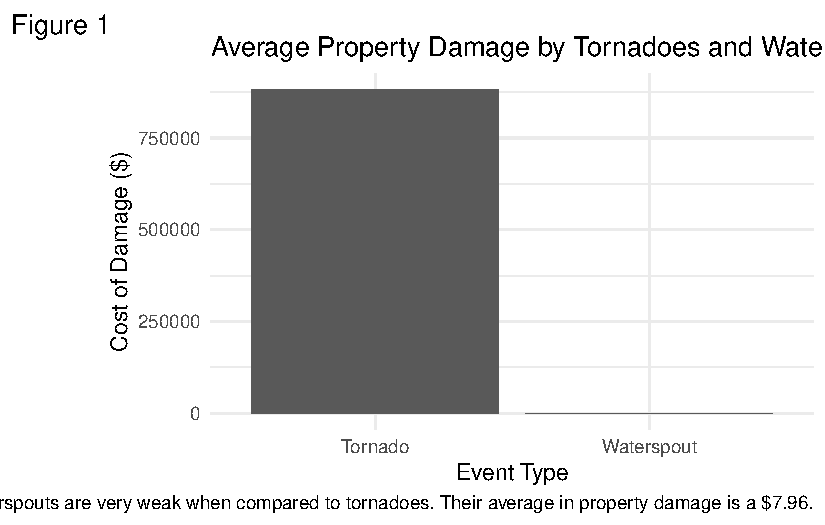
\includegraphics{draft-results2_files/figure-pdf/Average Property Damage Caused by Tornadoes vs Waterspouts Chart-1.pdf}

\textbf{Tornadoes that are strong enough to carry the weight of sharks
do not typically form near the coasts.}

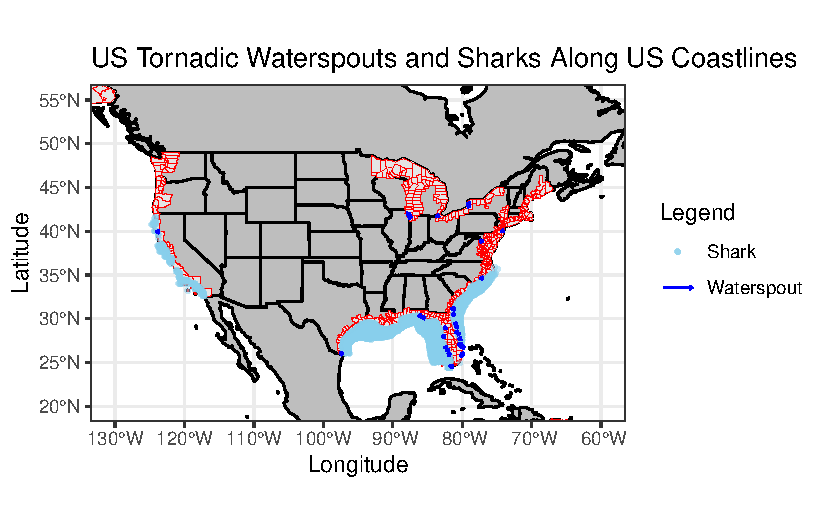
\includegraphics{draft-results2_files/figure-pdf/Path of Waterspouts in the US-1.pdf}

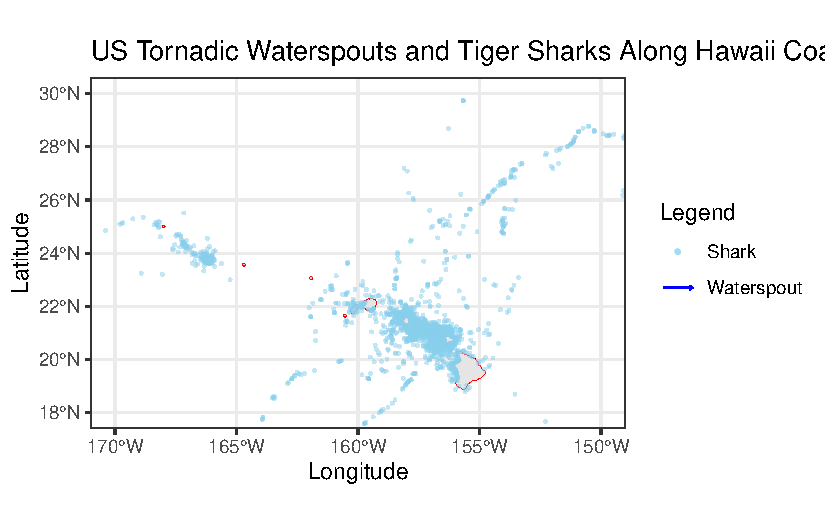
\includegraphics{draft-results2_files/figure-pdf/Path of Waterspouts in the US-2.pdf}

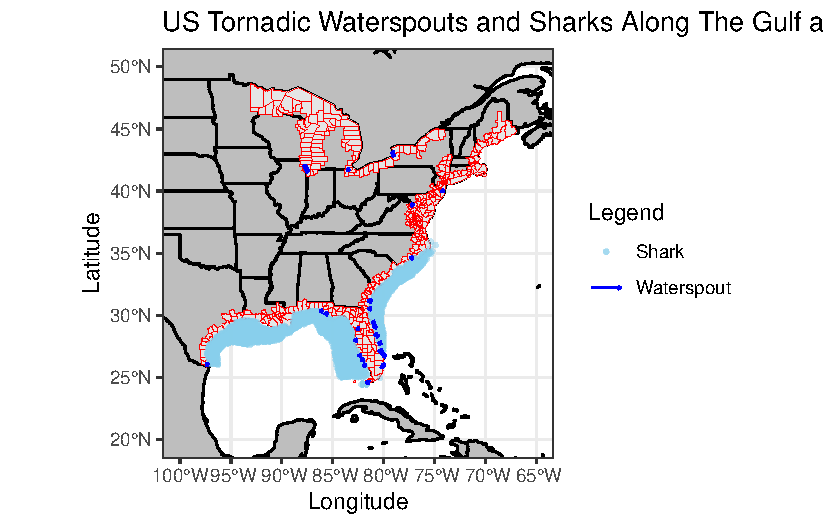
\includegraphics{draft-results2_files/figure-pdf/Path of Waterspouts in the US-3.pdf}

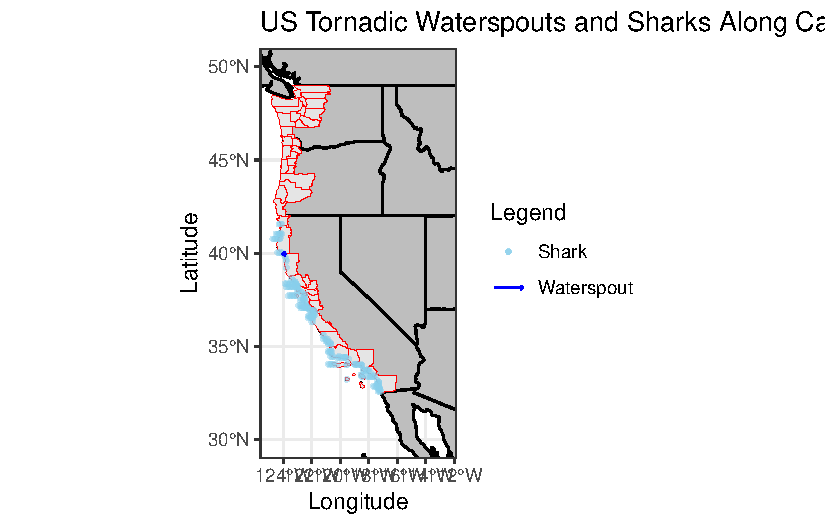
\includegraphics{draft-results2_files/figure-pdf/Path of Waterspouts in the US-4.pdf}

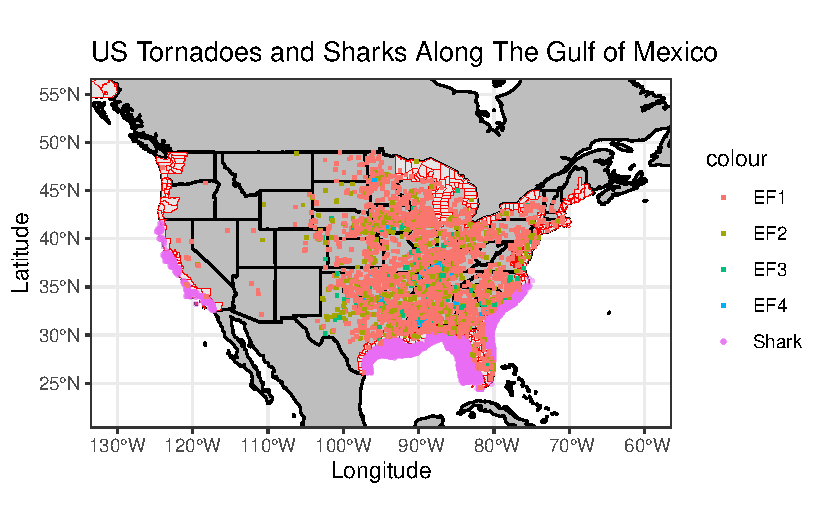
\includegraphics{draft-results2_files/figure-pdf/Path of Tornadoes in the US-1.pdf}

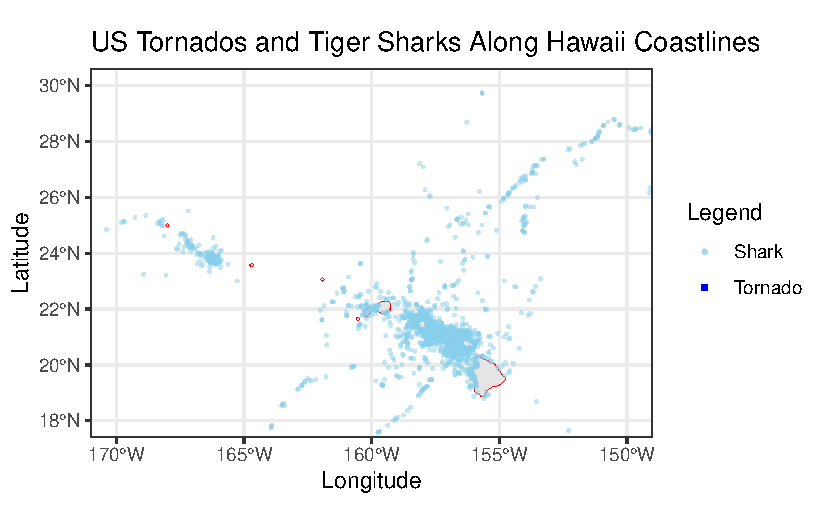
\includegraphics{draft-results2_files/figure-pdf/Path of Tornadoes in the US-2.pdf}

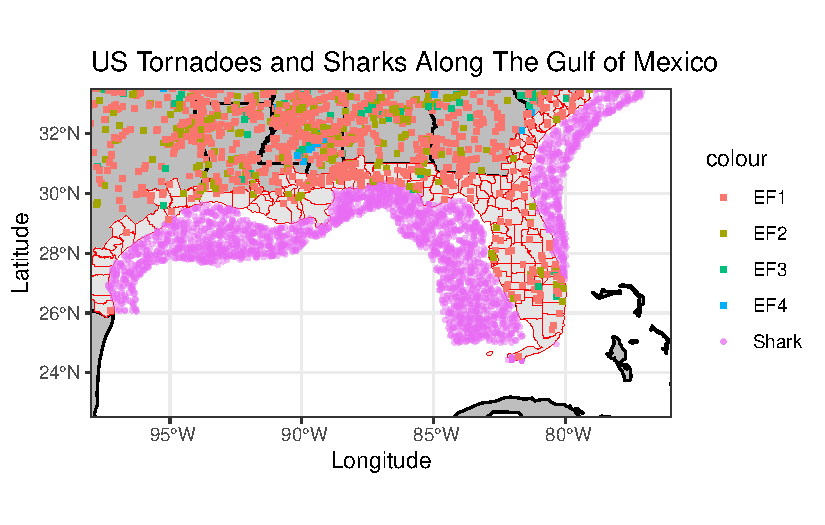
\includegraphics{draft-results2_files/figure-pdf/Path of Tornadoes in the US-3.pdf}

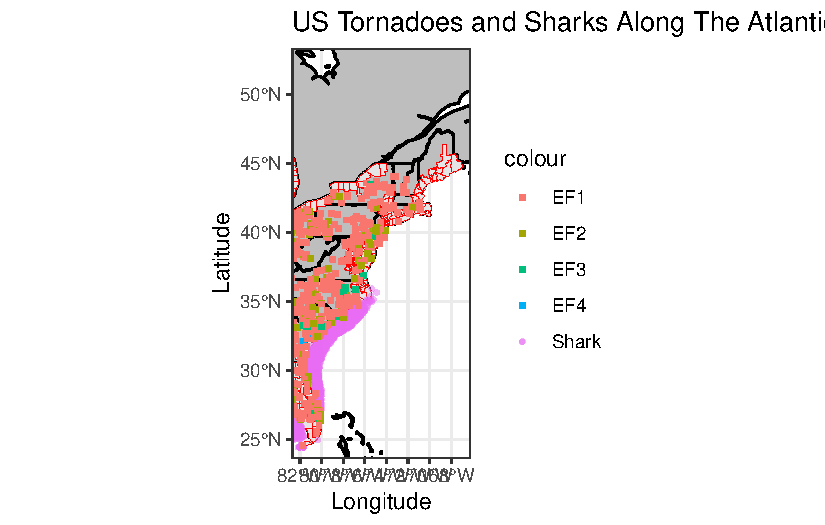
\includegraphics{draft-results2_files/figure-pdf/Path of Tornadoes in the US-4.pdf}

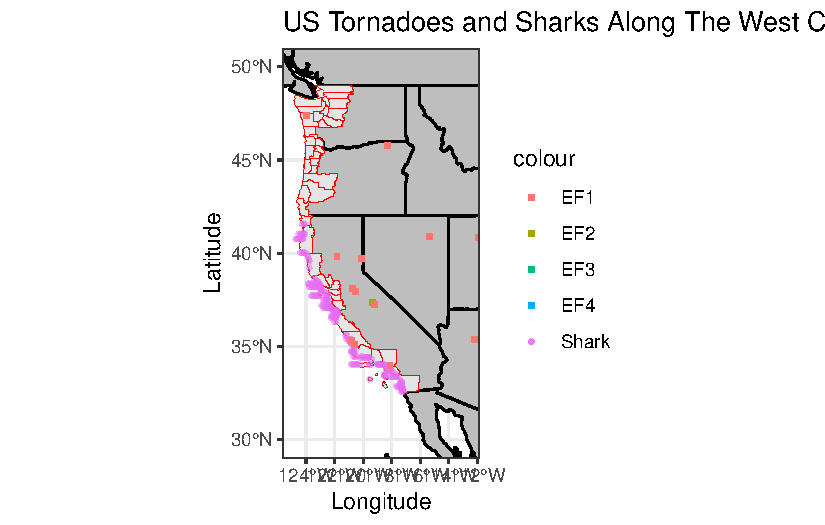
\includegraphics{draft-results2_files/figure-pdf/Path of Tornadoes in the US-5.pdf}

\begin{verbatim}
Observed Proportion of EF4 tornadoes: 0.0021 
\end{verbatim}

\begin{verbatim}
Observed Percentage of EF4 tornadoes: 0.21 %
\end{verbatim}

\textbf{Under the assumption that if an EF4 or EF5 tornado forms near
the coast, they will become sharknados, the likelihood that would happen
is very low}

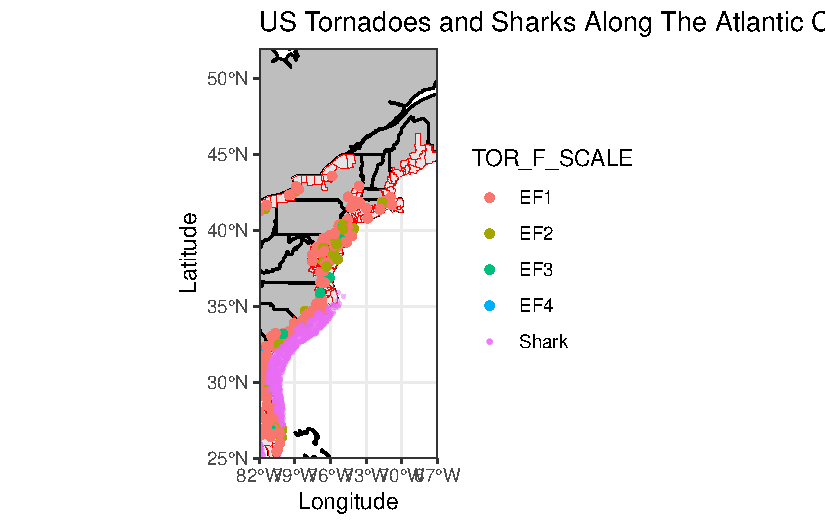
\includegraphics{draft-results2_files/figure-pdf/Checking only coastal tornadoes-1.pdf}

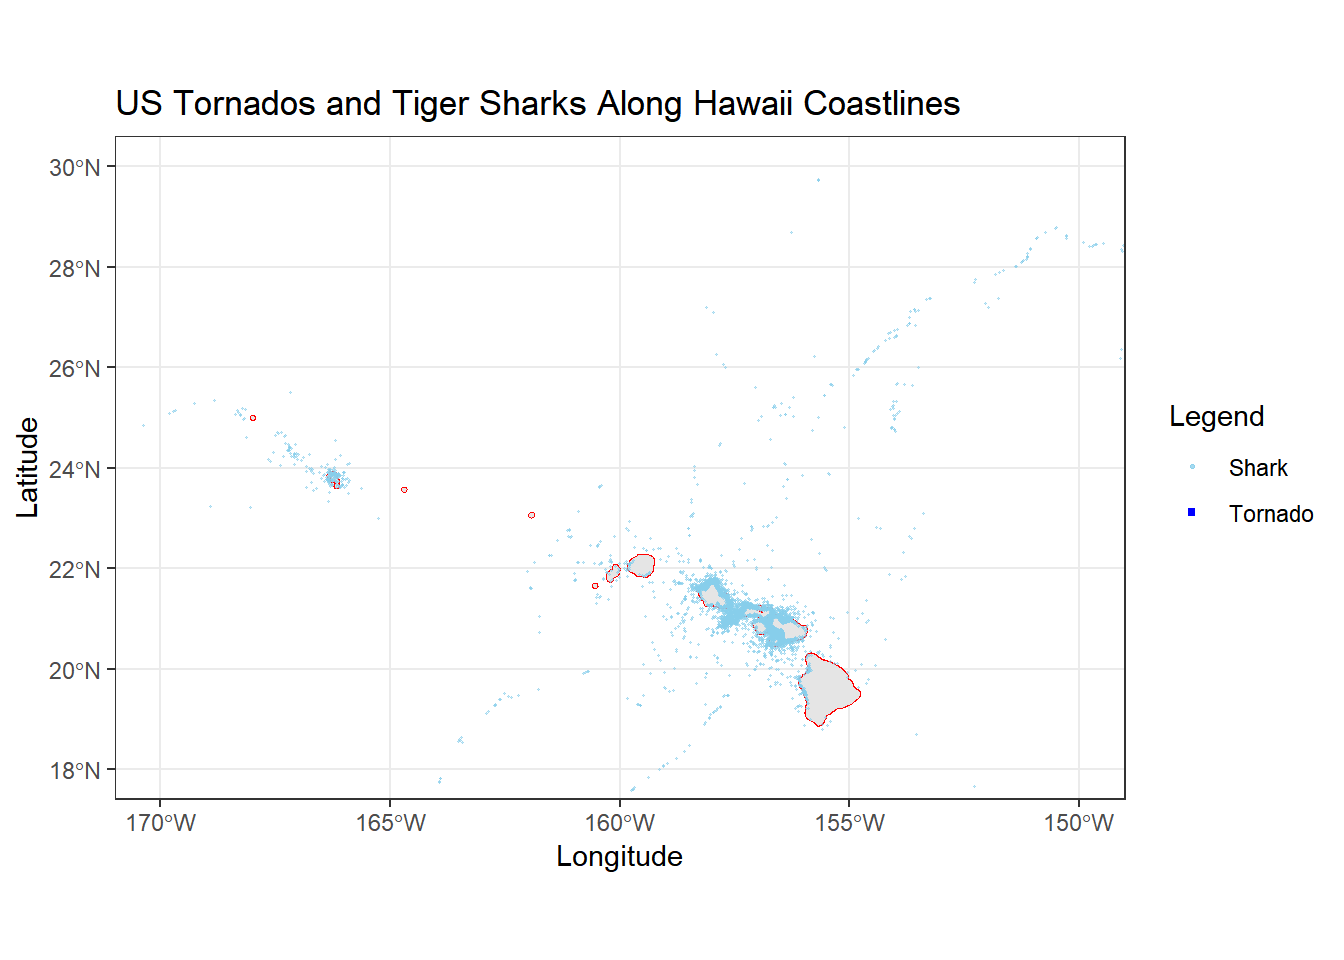
\includegraphics{draft-results2_files/figure-pdf/Checking only coastal tornadoes-2.pdf}

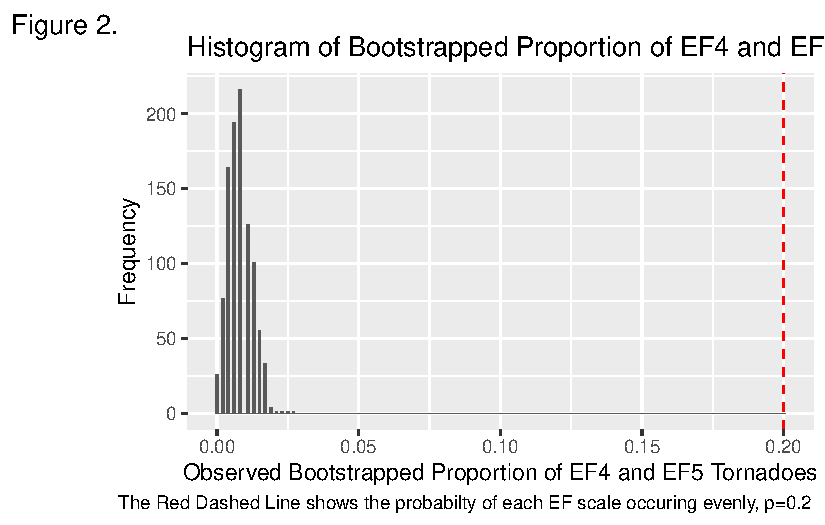
\includegraphics{draft-results2_files/figure-pdf/Bootstrap Sampling-1.pdf}

\begin{verbatim}
[1] 0
\end{verbatim}

\begin{verbatim}
[1] 0.008071882
\end{verbatim}

\begin{verbatim}
One-tailed p-value: 0 
\end{verbatim}

Given these very specific conditions: sharks are swimming close to the
surface of the ocean. An EF5 tornado is the only tornado would be needed
to carry sharks such as the hammerhead, tiger, and white shark. Given
that there is no EF5 tornado observed in the data and EF4 tornadoes are
also known to launch cars a considerable distance, we can assume that
EF4 tornadoes will become sharknados when formed near the coast.

Assuming each tornado is independent of each other, and there EF scales
are identically distributed, meaning that the relationship between EF
scale and location is random. A bootstrap sample can be done to test
that the probability of an EF4 tornado forming on the coast will happen
at random, meaning that there is a chance that a tornado powerful enough
to carry sharks (given the right conditions) will theoretically happen
at random.

A null hypothesis of Ho: p = 0.20 is made. This null states that the
probability of a EF4 tornado is equal to 20\%, that also means all 5
categories have an equal chance of occurring. An alternative hypothesis
states Ha: p \textless{} 0.20, meaning the chance of a tornado being an
EF4 tornado on the coast is less than 0.20.

The observed proportion of EF4 tornadoes in our data is 0.0021 meaning,
that in our observed sample, it is very unlikely for EF4 tornadoes to
form near the coast. When bootstrapping, a bootstrapped observed
proportion of EF4 tornadoes is 0.0080719. The tells us that the
probability of our observation happening at random is approaching very
closely to 0.

We do not have enough evidence to say that these EF4 and EF5 tornadoes
appear on the coasts at random, so we must reject that idea and can
confirm that it is not likely that tornadoes with the potential to cause
shark-infested terror will be a threat people should be worried about in
the future.

\chapter{Draft: Intro/Conclusions}\label{draft-introconclusions}

\chapter{Introduction}\label{introduction-1}

\section{A Real Life Sharknado?}\label{a-real-life-sharknado}

There is a growing concern over the possibility of a real life
\emph{Sharknado}, a tornado that forms over water, gathers sharks in its
powerful vortex, and then travels onto land, carrying the sharks with
it. These sharknados wreak havoc all throughout the United States in
locations like Los Angeles, New York City, and even Washington D.C. all
the way down to Orlando, Florida raining sharks down from the sky. There
have been circumstances where tornadoes have picked up animals such as
fish and frogs, if one's imagination is not limited, one could see it be
possible for tornadoes to carry sharks. Although this concept originates
science fiction movie series, it raises serious questions on how thin
the line between fiction and reality might be when it comes to such a
catastrophic event.

\section{Tornadoes and Sharks}\label{tornadoes-and-sharks}

To help figure out how a \emph{sharknado} would be possible, the
strenghts and conditions of tornadoes must be analyzed to see how they
could carry these apex marine predators.

\subsection{How Strong can a Tornado
Be?}\label{how-strong-can-a-tornado-be}

The Enhanced Fujita Scale (EF Scale), which is used to assign a tornado
a rating based on estimated wind speeds. The scores and their estimated
wind speeds go as follows:

\section{Enhanced Fujita (EF) Scale and Wind
Speeds}\label{enhanced-fujita-ef-scale-and-wind-speeds}

\begin{longtable}[]{@{}ll@{}}
\caption{Table: Enhanced Fujita (EF) scale and corresponding wind
speeds}\tabularnewline
\toprule\noalign{}
EF\_Rating & Wind\_Speed\_Range \\
\midrule\noalign{}
\endfirsthead
\toprule\noalign{}
EF\_Rating & Wind\_Speed\_Range \\
\midrule\noalign{}
\endhead
\bottomrule\noalign{}
\endlastfoot
EF0 (Weakest) & 65 - 85 mph \\
EF1 & 86 - 110 mph \\
EF2 & 111 - 135 mph \\
EF3 & 136 - 165 mph \\
EF4 & 166 - 200 mph \\
EF5 (Strongest) & Over 200 mph \\
\end{longtable}

Minor damage such as broken tree branches and roof shingles being blown
away can be expected from EF0 tornadoes. While on the other end of the
spectrum, EF5 tornadoes can promise wind speeds that can decimate well
built homes and infrastructure. These tornadoes can carry objects like
cars with no trouble. An EF2 tornado is where we finally see enough
force for winds to pick up a small car around 2000lbs, but not enough
force for it to be thrown wildly. In the center, an EF3 tornado can
remove the roofs off buildings on uproot small trees. An EF4 tornado is
where we finally begin to see heavy objects such as trucks, cars, and
semis be thrown around considerable distances.

An EF5 tornado will for sure have the potential to be a
\emph{sharknado,} and another contender is the EF4 tornado and maybe, if
the conditions are just right, an EF3 tornado might be able to, however,
this is being very generous. Our \emph{sharknado} would realistically
have to be a category EF5 or EF4 tornado in order to cause terror
similar to the film.

\subsection{Tornado or Waterspout?}\label{tornado-or-waterspout}

This \emph{sharknado} would need to have a tornado that forms over shark
infested waters. A tornado that forms over water is usually classified
as a waterspout. Waterspouts are not classified as tornadoes, so they
are not given a score on the EF scale. If a waterspout moves on shore
however, The National Weather Service classifies it as a tornado and
issues a tornado warning for the area.

Waterspouts are generally broken into two categories: fair weather
waterspouts and tornadic waterspouts. Fair weather waterspouts to put it
simply are a less dangerous event that form during relatively calm
weather and are not associated with thunderstorms. The phenonema of
interest are tornadic waterspouts. These have the same characteristics
of a land tornado, they are often accompanied by high winds, severe
thunderstorms, large hail. It is essentially a tornado that forms over
water, but it can also form by a tornado moving from land to water. If a
\emph{sharknado} would occur this is how it would form!

\subsection{Sharks in Infested Waters in the United
Sates}\label{sharks-in-infested-waters-in-the-united-sates}

Sharks are found in coastal waters along the East Coast, Gulf of Mexico,
and the Caribbeans. These waters are where a \emph{sharknado} would have
to form.

Sharks vary greatly in size and weight. Some common sharks and their
average adult weights include:

\begin{longtable}[]{@{}ll@{}}
\caption{Table: Shark species and typical weight ranges}\tabularnewline
\toprule\noalign{}
Species & Weight\_Range\_lbs \\
\midrule\noalign{}
\endfirsthead
\toprule\noalign{}
Species & Weight\_Range\_lbs \\
\midrule\noalign{}
\endhead
\bottomrule\noalign{}
\endlastfoot
Atlantic Sharpnose & 15 - 25 \\
Atlantic Blacktip & 66 - 200 \\
Tiger & 850 - 1400 \\
Hammerhead & 500 - 1000 \\
Sandtiger & 200 - 350 \\
The Great White & 1500 - 2400 \\
\end{longtable}

The sharks that were commonly seen inside the \emph{sharknado} were the
tiger shark, the hammerhead shark, and of course, the great white shark.

\section{Can a Sharknado Actually
Occur?}\label{can-a-sharknado-actually-occur}

Is it possible to predict if a \emph{sharknado} can happen in real life
using exisiting data about sharks and tornadoes from years past?

To answer this burning question, a scrutinizing look at meteorological
and marine data must be done.

\chapter{Conclusions}\label{conclusions}

\section{\texorpdfstring{Tornadic Waterspouts Powerful Enough to Carry
Sharks \emph{And} Makes Landfall is an Unlikely
Event}{Tornadic Waterspouts Powerful Enough to Carry Sharks And Makes Landfall is an Unlikely Event}}\label{tornadic-waterspouts-powerful-enough-to-carry-sharks-and-makes-landfall-is-an-unlikely-event}

Key findings suggest that a sharknado is not likely to occur.
Waterspouts do tend to form in shark infested waters, but these are not
powerful enough to lift sharks that can weight up to 2400 lbs and
relocate them to land. From the more powerful of the two types of
waterspouts, tornadic waterspouts' power are limited and never seem to
make landfall.

\subsection{There is a Little Amount of Tornadoes with a High Enough EF
Scale that form near the
coasts}\label{there-is-a-little-amount-of-tornadoes-with-a-high-enough-ef-scale-that-form-near-the-coasts}

Tornadoes that do form near the coasts typically have an EF rating of
EF2 or lower. An EF2 tornado \emph{has} the power to lift a car and move
it a ways from where it was, but when trying to find the possibility of
lifting sharks throughout a city, a stronger EF4 tornado is very well
needed to pull the sharks from the depths of the water. Although there
are some EF3 tornadoes present in Florida, and EF3 tornadoes could pick
up a car and throw them a considerable distance, the chance that sharks
are swimming near the surface of the water to be pulled into the vortex
is low. There is an EF4 tornado located in Georgia, however this tornado
is not close enough to the ocean coasts that it would be able to make
contact with the sharks present there.

\section{Real World Interpretation}\label{real-world-interpretation}

People of the United States that live on the coasts can be clear of mind
that a sharknado will not be one of their worries when it comes to
weather events such as hurricanes and tropical storms.

\section{Limitations in Data and
Knowledge}\label{limitations-in-data-and-knowledge}

\subsection{No Free Shark Survey Dataset (From a Trusted Source) that
Has Observations on the West Coast or Northeast of
America}\label{no-free-shark-survey-dataset-from-a-trusted-source-that-has-observations-on-the-west-coast-or-northeast-of-america}

Although our data showed that tornadic waterspouts and tornadoes that
form near the coasts of America do not form too often and are not that
powerful, there was not much comparison when plotting those events
against sharks surveyed or spotted outside of the Southeast or Hawaii.
Data for California was found, however that was not survey or tracking
data, rather it was shark incident data. This leads to more sharks being
plotted in places that have more people, preventing an evenly
distribution of shark points on the map. Due to this limitation, our
interpretation can only be justified that people on the coasts of the
Southeast region of America near the Gulf of Mexico, Hawaii, and
California.

\subsection{Bootstrapping}\label{bootstrapping}

Our probability observed from our bootstrapped sample of 0.008, only
tells us that if the EF scales of the tornadoes in our dataset were
randomized, and they were measured on the tornadoes near the coasts,
that is the long run proportion of EF4 and EF5 tornadoes that will form
near the coasts. However, the way the coastal data is set up, these
tornadoes can be technically in the coastal region plotted, but be too
far away from the coastline to be able to cause havoc with sharks. Our
bootstrap probability is then not really the true average amount of
tornadoes that would be able to lift sharks, and in reality it could be
greater or it could be less.

\subsection{Hurricanes?}\label{hurricanes}

In this report, only tornadoes were considered. This can be a bit
problematic when looking at a place like Hawaii. There are very little
tornadoes recorded in Hawaii, yet a lot of sharks. It could be argued,
that a hurricane of great strength could be enough to lift the numerous
sharks surrounding Hawaii, but in as stated previous, we are not
interested in \emph{Shark-icanes}.

\subsection{Comparing Tornadoes and
Waterspouts}\label{comparing-tornadoes-and-waterspouts}

Waterspouts do not have any classification of power similar to
tornadoes. There in order to compare the differences in power between
the two, the observed damage to property was looked at. A problem with
this is that waterspouts will most likely be less damaging as they are
not near much property at all when forming. This caused the averages to
be compared instead, but there is still some limitations on how far the
implication of just how strong waterspouts can be.

\section{Future Directions and
Implications}\label{future-directions-and-implications}

If a budget allows, using private data may be able to help know just how
close these coastal tornadoes and tornadic waterspouts are to the shark
population of America.

\chapter{Draft: Executive Summary}\label{draft-executive-summary}

The Sharknado film series takes the idea of tornadoes picking up marine
life to a dramatic extreme. While there has not been a documented case
of a tornado hurling sharks onto land, we explored whether such an event
is even scientifically plausible. We examined whether powerful tornadoes
could form over or near coastal shark-infested waters, lift sharks into
the air, and carry them inland.

To assess the likelihood of a tornado capturing sharks within its vortex
and terrorizing the public, we analyzed tornado data from 2020 to 2024
and shark population data near U.S. coastlines, particularly around the
Gulf of Mexico. We defined three key conditions that are required for a
Sharknado to occur: (1) a tornado must be strong enough to lift a shark,
(2) it must form over or near shark-inhabited waters, and (3) it must
move inland.

Our findings indicate that waterspouts, tornadoes that form over water,
are generally weaker than their land-based counterparts and are unlikely
to lift large animals such as sharks. On the other hand, stronger
tornadoes typically do not form directly over water or in close
proximity to shark habitats. The two types of tornadoes with the
potential to lift sharks from the water are EF4 and EF5 tornadoes given
the very specific conditions that sharks are near the surface of the
water. Assuming that if tornadoes form relatively near the coasts of the
United States and shark-inhabited waters, the observed probability of
EF4 and EF5 tornadoes forming on the coast is 0.0021. When bootstrapping
under the assumption that each scale of tornado has an equal chance of
happening ( Null: p = 0.2 ), we get an observed bootstrap average of
0.008.

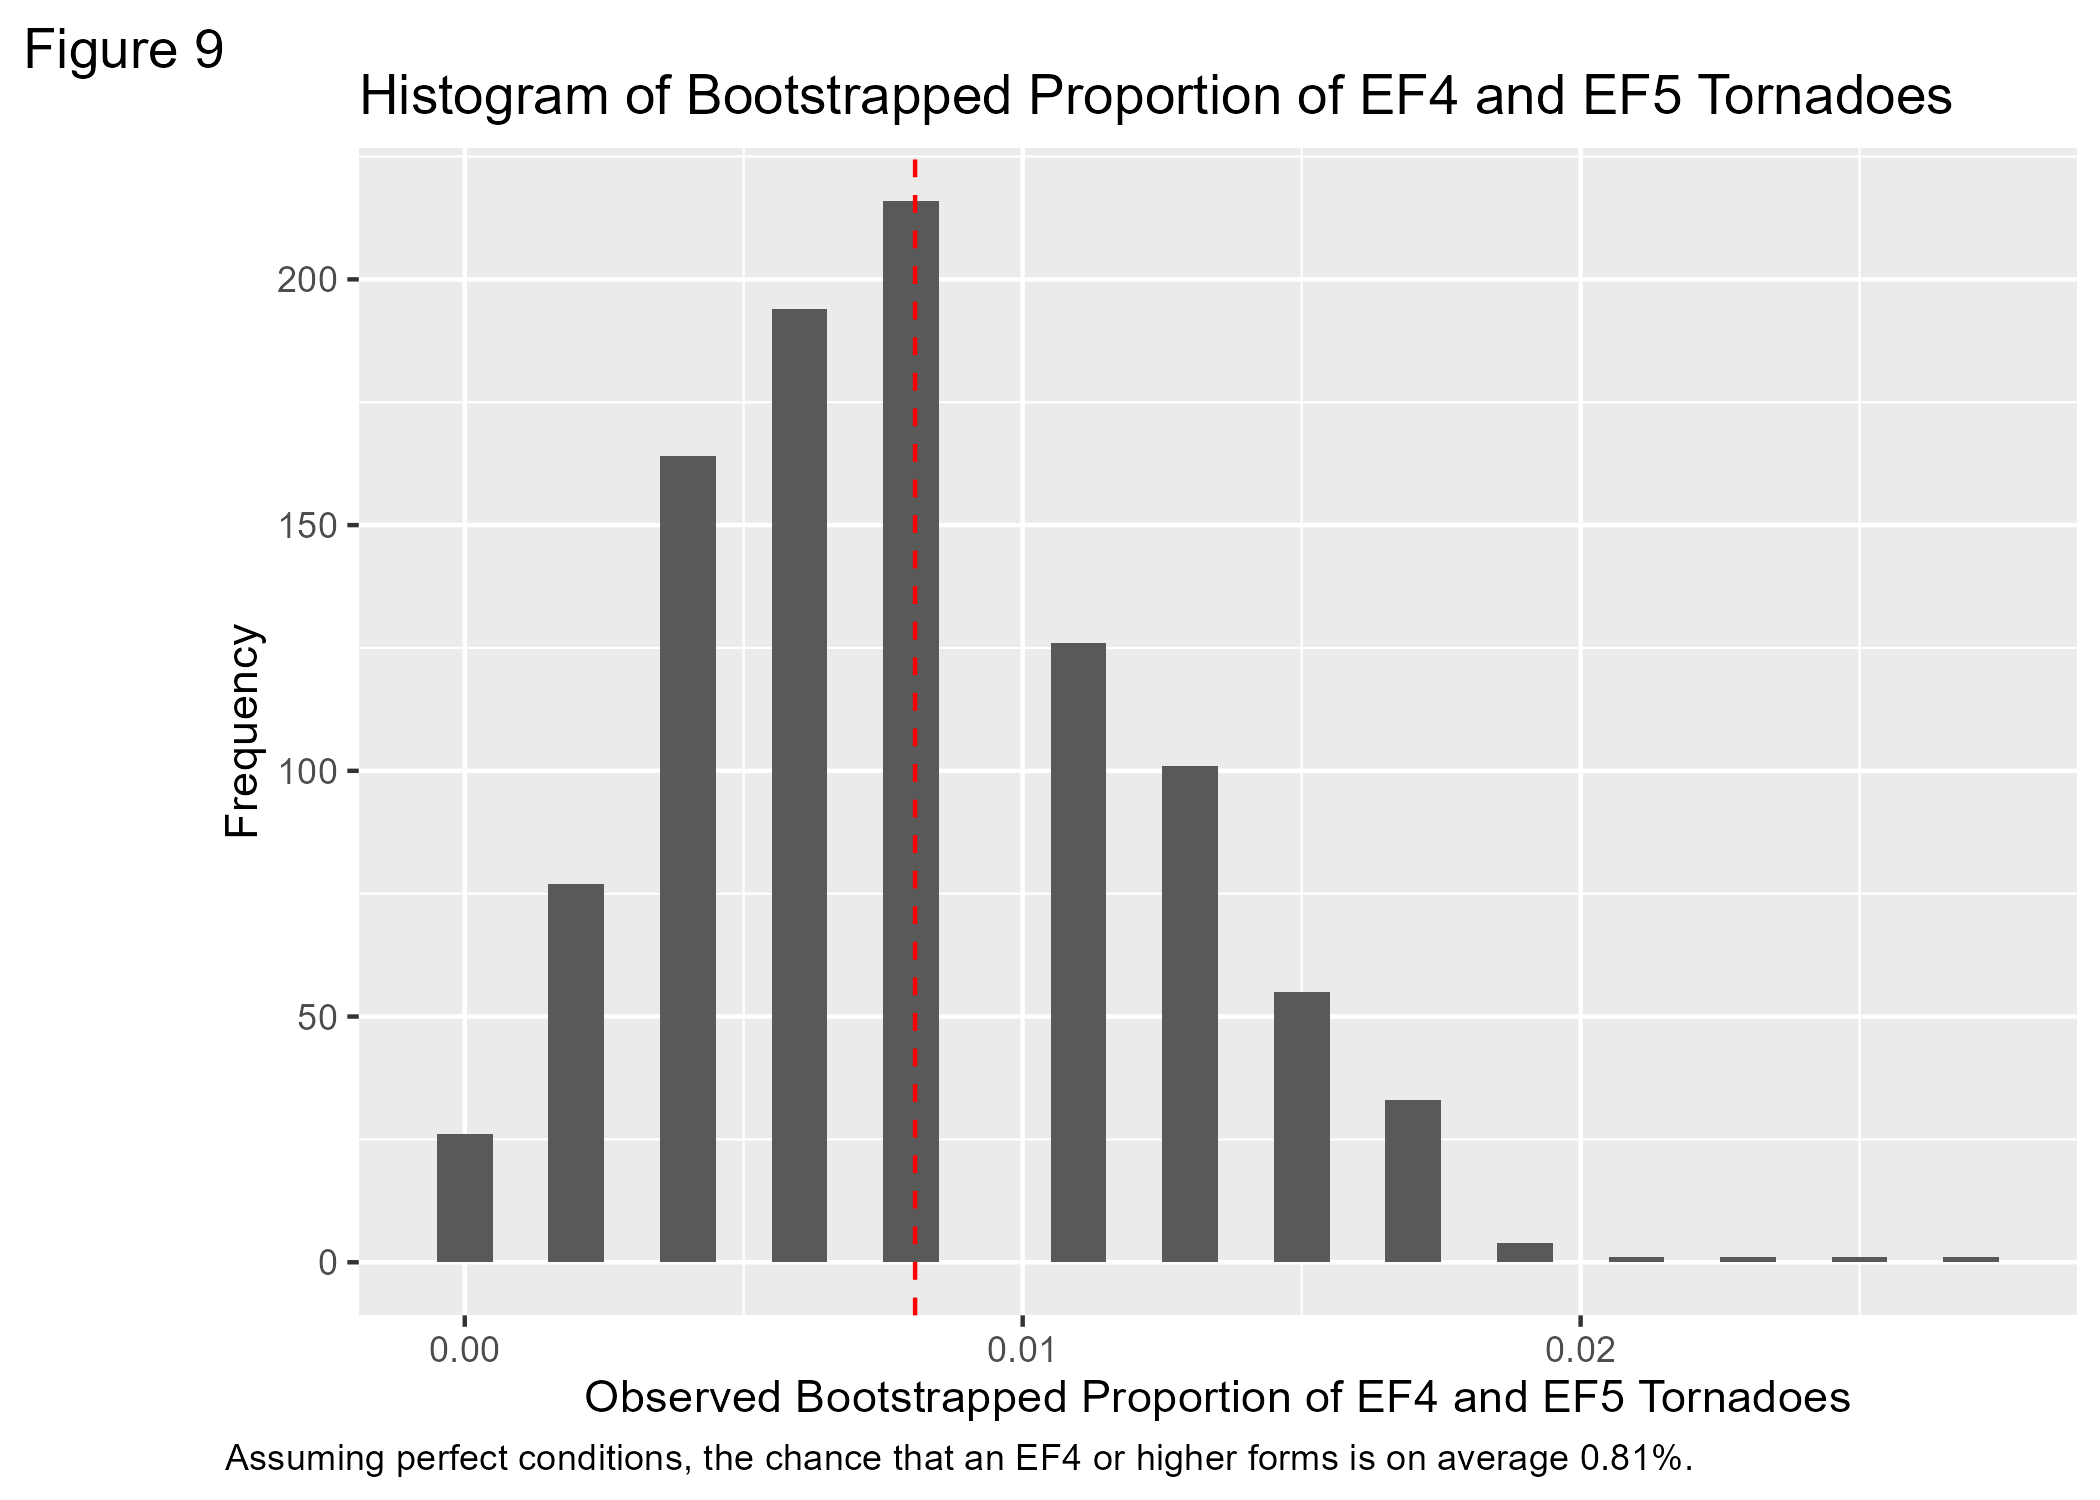
\includegraphics{bootstrap_histogram.png}

Therefore, while the Sharknado scenario remains a thrilling fictional
concept, the probability of such an event occurring any time soon in
real life is extremely low.



\end{document}
